% !TeX root = ../index.tex
\chapter{Design}
\graphicspath{{2-design/images/}}

The app has three main pages that users interact with - the notes list that is shown when the app is launched, the note(s) itself and a settings page to alter the default preferences. I designed several proof-of-concept designs for what the app could look like using MockFlow.

Below are annotations to the six numbered mock-ups on the following pages:
\begin{enumerate}
  \item[2.1.1] The notes are displayed in a list with the note title and the time since the note was last modified. The time shown as a relative (30 minutes) or absolute (26 Apr '18) could potentially be an option toggleable in the settings page. Clicking a note should take the user to the note page.

  \item[2.1.2] Clicking the Floating Action Button in \textbf{2.1.1} should prompt the user to enter a name for their new note.

  \item[2.2.1] The note page allows the user to view or edit their notes. The note title is displayed in the toolbar with the two icons on the right for editing the note title and saving the note. Backing out of the note with unsaved changes could prompt the user asking if they wish to save or discard the changes.

  \item[2.2.2] The settings page should allow the user to change the app language, theme (e.g light, dark or AMOLED) and where the notes are saved.

  \item[2.3.1] This is a revision of \textbf{2.1.1} where I moved the modification date to below the note title and removed the abbreviations.

  \item[2.3.2] The final revision of \textbf{2.1.1} after looking through the Activity templates the latest Android Studio provides. This adopts the large toolbar and moves the Floating Action Button up to the top. This should improve one-handed use on larger devices where most of this screen's activity will occur in the top half. While no longer an issue as I had previously relocated the time text, the FAB in the bottom right would also have obscured the text on notes at the bottom of the screen.
\end{enumerate}

\begin{figure}[H]
  \begin{subfigure}{.5\textwidth}
    \caption{Mockup of the start page}
    \centering
    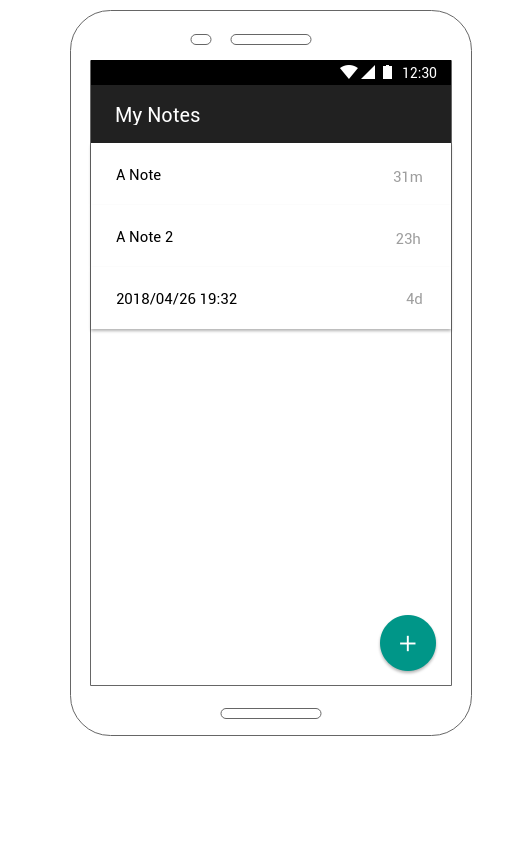
\includegraphics[width=\textwidth]{mockup-list}
  \end{subfigure}
  \begin{subfigure}{.5\textwidth}
    \caption{Mockup of creating a new note}
    \centering
    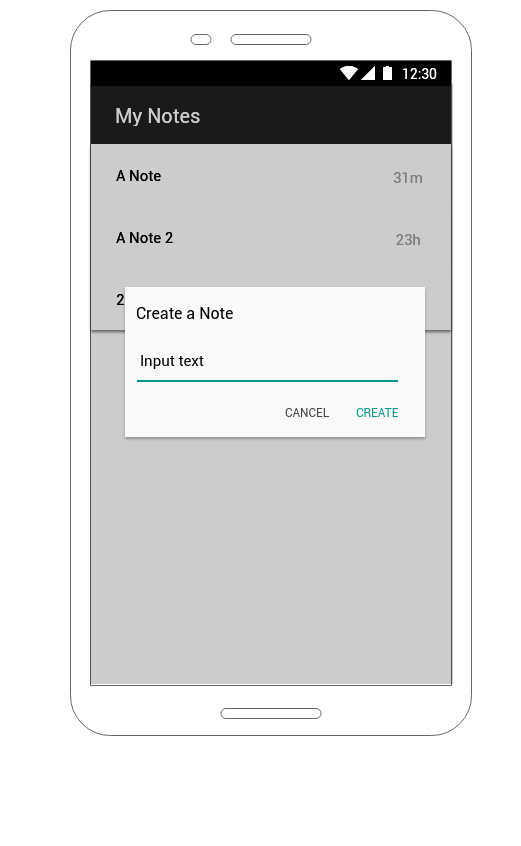
\includegraphics[width=\textwidth]{mockup-new}
  \end{subfigure}
\end{figure}

\begin{figure}[H]
  \setcounter{subfigure}{2}
  \begin{subfigure}{.5\textwidth}
    \caption{Mockup of the note editing page}
    \centering
    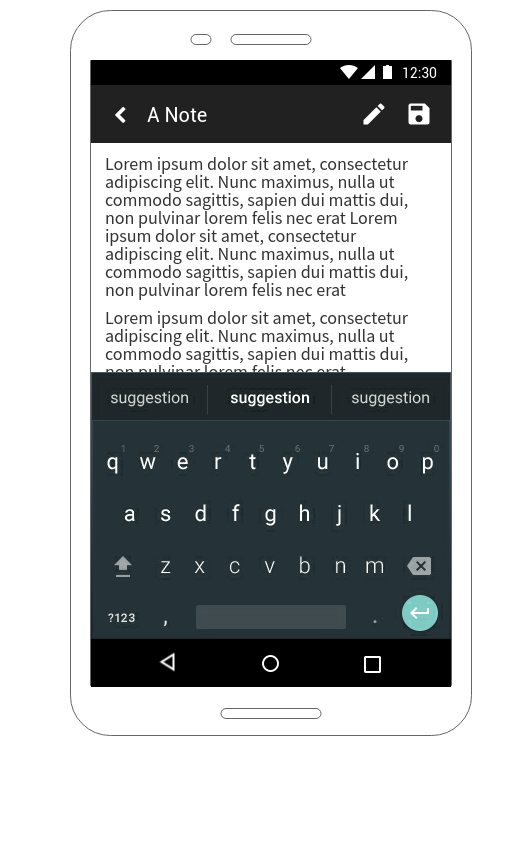
\includegraphics[width=\textwidth]{mockup-note}
  \end{subfigure}
  \begin{subfigure}{.5\textwidth}
    \caption{Mockup of the settings page}
    \centering
    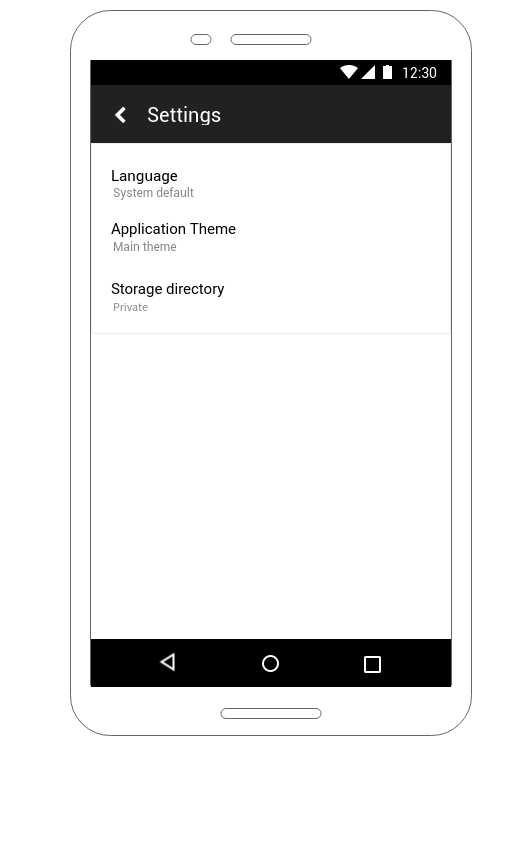
\includegraphics[width=\textwidth]{mockup-settings}
  \end{subfigure}
\end{figure}

\begin{figure}[H]
  \setcounter{subfigure}{2}
  \begin{subfigure}{.5\textwidth}
    \caption{Revised mockup of the start page}
    \centering
    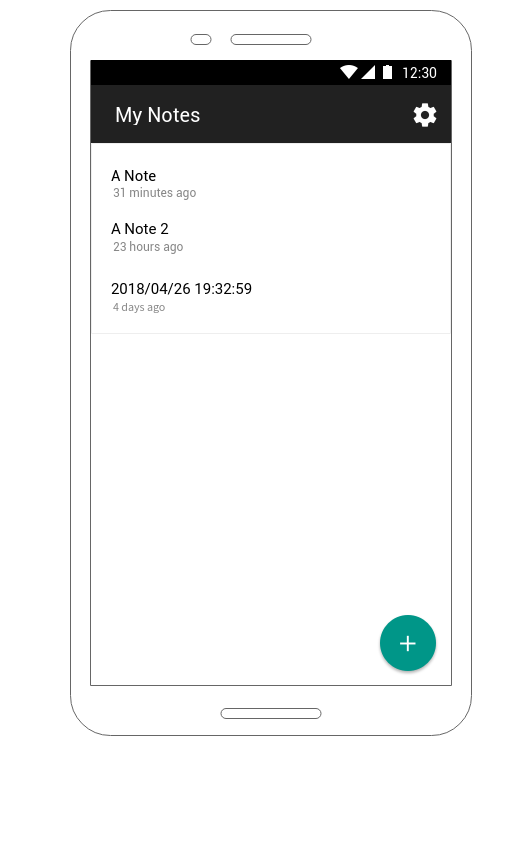
\includegraphics[width=\textwidth]{mockup-list2}
  \end{subfigure}
  \begin{subfigure}{.5\textwidth}
    \caption{Revised mockup of the start page}
    \centering
    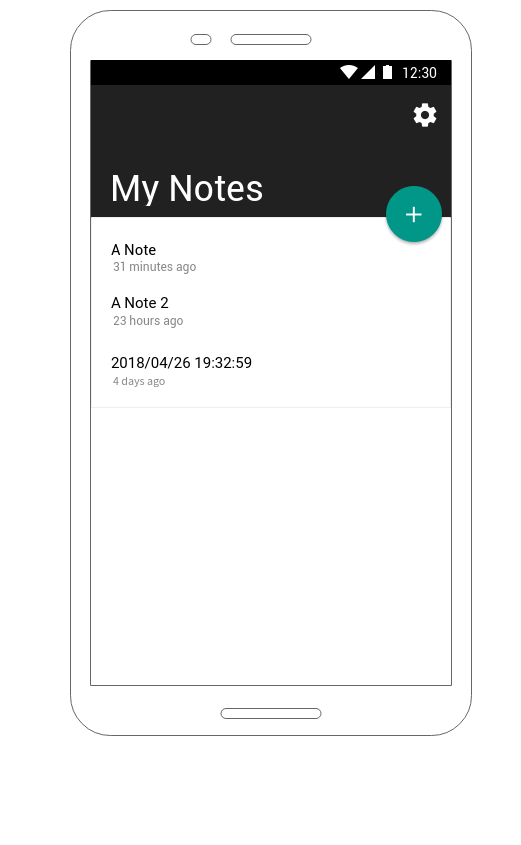
\includegraphics[width=\textwidth]{mockup-list3}
  \end{subfigure}
\end{figure}

%You need to develop an App idea, this need not be unique but might be based on an app you currently use or have seen used with a functionality adaptation.  Maybe you will consider a ‘mash-up’ of other ideas you have come across.  The main point here is to consider your idea within a market segment then design, implement, test and publish your app on a mobile device or a mobile device emulator running on a computer.

%You are required to produce a brief report covering the background to the app idea covering the design, implementation, testing and publishing of your App.  The main salient aspects should be discussed e.g. various supporting stages of the development process, problems and how they were overcome, USP (unique selling point) etc. Please remember you need to justify any decisions/choices made in your design/development.
